\documentclass[12pt]{article}
\usepackage[utf8]{inputenc}	
\usepackage[catalan]{babel}
\usepackage{subcaption}
\usepackage[obeyspaces]{url}
\usepackage[colorinlistoftodos]{todonotes}
\usepackage[]{mcode}
\usepackage{fancyvrb}
\usepackage{eurosym} %Símbol del euro
\usepackage[obeyspaces]{url} %PATH
\usepackage{wrapfig} %Imatges WRAP (mateixa linia)
\usepackage[toc,page]{appendix}
\usepackage{todonotes}
\usepackage{appendix}
\usepackage{scrextend}
\usepackage{enumitem}
\usepackage{dirtytalk}
\usepackage{multicol}
\usepackage{listingsutf8}
\usepackage{dirtytalk}
\usepackage{float}
\usepackage{url}
\setlength{\parindent}{0cm} \setlength{\oddsidemargin}{-0.5cm} \setlength{\evensidemargin}{-0.5cm}
\setlength{\textwidth}{17cm} \setlength{\textheight}{23cm} \setlength{\topmargin}{-1cm} \addtolength{\parskip}{2ex}

\definecolor{backcolour}{rgb}{0.95,0.95,0.92}
\lstdefinelanguage{json}{
	backgroundcolor=\color{backcolour},   
	breaklines=true, 
    string=[s]{"}{"},
    stringstyle=\color{blue},
    comment=[l]{:},
    commentstyle=\color{black}
}

\definecolor{mygreen}{rgb}{0,0.6,0}
\definecolor{mygray}{rgb}{0.5,0.5,0.5}
\definecolor{mymauve}{rgb}{0.58,0,0.82}

\lstset{
	backgroundcolor=\color{backcolour},   
	breaklines=true, 
	numbers=left,
	basicstyle=\footnotesize,
	commentstyle=\color{mygreen},    % comment style
  escapeinside={\%*}{*)},          % if you want to add LaTeX within your code
  keywordstyle=\color{blue},       % keyword style
  stringstyle=\color{mymauve},     % string literal style
}

\renewcommand{\baselinestretch}{1.5}

\begin{document}
\begin{titlepage}
		\centering
		\includegraphics[width=0.5\textwidth]{imatges/logo3.png}\par\vspace{1cm}
		{\huge\bfseries Posicionament de restaurants\par}
		\vspace{0.3cm}
		{\scshape\Large Processament de Dades Espaials\par}
		\vspace{0.2cm}
		{\scshape\Large Màster en enginyeria informàtica\par}
		\vspace{1.5cm}
		{\Large\itshape Oscar Galera Alfaro i Meriem Abjil Bajja\par}
		\vfill
		{\large \today\par}
\end{titlepage}
\tableofcontents

\clearpage

\listoffigures

\clearpage

\section{Introducció}

Els dissenyadors de \textit{Disney Land París} han descobert com mantenir el seu univers feliç: mitjançant l'ús de polseres \textit{Magic Bands} per fer un seguiment de les identitats, els moviments i l'estat financer dels usuaris.

El \textit{MyMagic } + \say{sistema de gestió de vacances} pot fer un seguiment dels convidats a mesura que es mouen per \textit{Disney Land París} i analitzar els seus hàbits de compra.

Degut a l'èxit generat per \textit{Disney Land París} (a partir d'ara \textit{DPL}), el propietari d'aquest ha decidit obrir un nou parc temàtic similar (veure \textit{Figura \ref{fig:disney1}}) però aquest cop en el territori Gironí. Ens han encarregat indicar el posicionament dels restaurants amb l'objectiu de maximitzar els beneficis generats per aquests. Per ubicar aquests restaurants, es realitzarà un estudi de la popularitat de les atraccions que hi ha a \textit{DLP} a fi de determinar les zones més visitades, i d'aquesta manera, fer la distribució dels restaurants més cars en aquestes zones per maximitzar els beneficis generals del parc.

%Posicionament de la imatge
\begin{figure}[H]
    \centering
    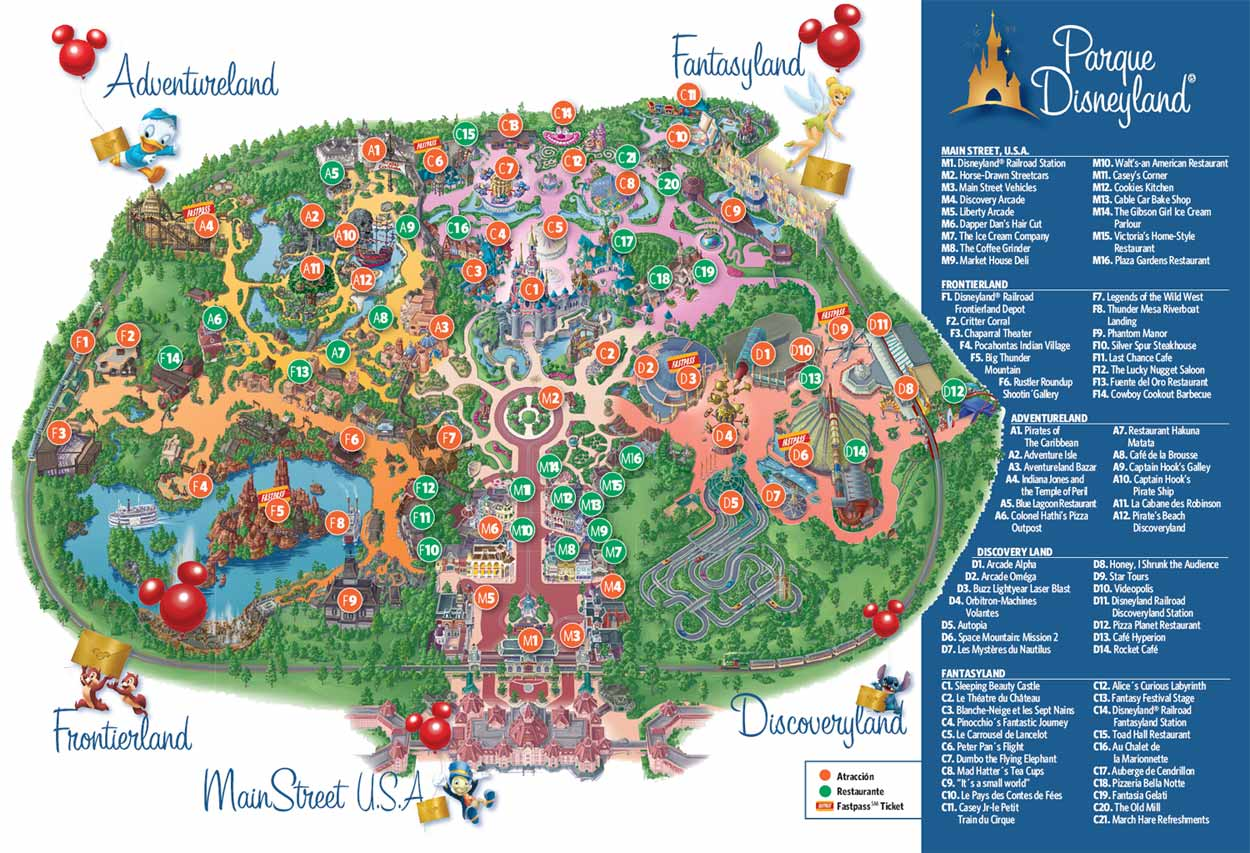
\includegraphics[width=0.75\textwidth]{imatges/mapa_disney_land_paris.jpg}\par\vspace{1cm}
    \caption{Mapa de \textit{Disney Land París}}
    \label{fig:disney1}
\end{figure}

\clearpage
\section{Objectiu}
L'objectiu del projecte és \textbf{fer la distribució dels restaurants més cars a partir d'unes determinades zones \say{remarcades} per maximitzar els beneficis del parc}. Aquestes zones les anomenarem \say{candidates}, i seran aquelles on es podran ubicar els restaurants.

Per aconseguir aquest objectiu es considerarà que el mapa d'atraccions del nou territori és el mateix que el de \textit{DLP}; que les \textit{Magic Bands} (veure \textit{Figura \ref{fig:magic_bands}}) recullen i emmagatzemen la informació de la posició dels seus usuaris cada 5 minuts, i que disposem de tantes zones candidates (o més) com restaurants es vulguin ubicar. 

Per determinar el grau d'interès de cada atracció, es compta amb una gran quantitat de dades generades per les \textit{Magic Bands} (veure \textit{Figura \ref{fig:magic_bands}}) que es reparteixen a l'entrada del parc temàtic, i que tenen per objectiu la recollida de dades públic a fi d'estudiar el seu comportament. 

\begin{figure}[H]
    \centering
    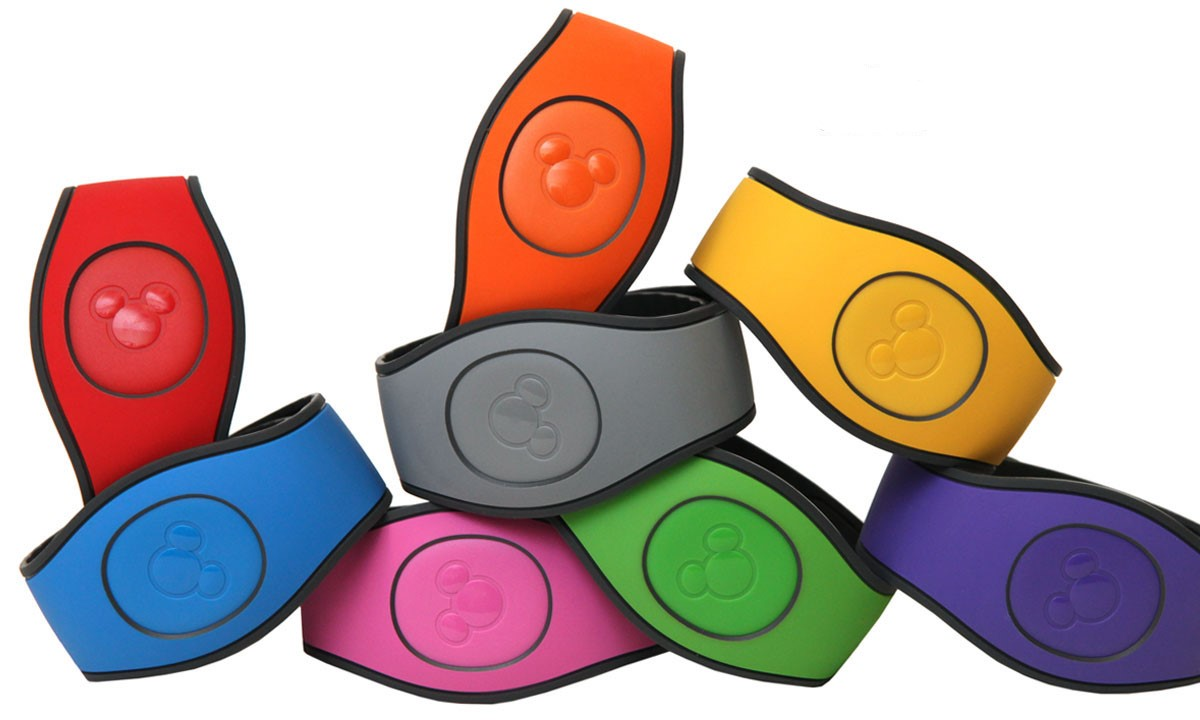
\includegraphics[width=1\textwidth]{imatges/magic_bands.jpg}
    \caption{\textit{Magic Bands}}
    \label{fig:magic_bands}
\end{figure}

\clearpage
\section{Definició del problema}
Per aconseguir l'objectiu que s'ha plantejat es seguiran 6 passos, que són:
\begin{enumerate}
	\item Preprocessament de dades (veure \textbf{secció \ref{pd}}).
	\item Filtrat de dades.
	\item Assignar un pes a cada atracció.
	\item Dividir el mapa en àrees.
	\item Definir les zones candidates.
	\item Ubicar els restaurants.
\end{enumerate}

S'assumeixen les següents entrades\footnote{Aquestes entrades vindran proporcionades per la direcció del parc}:
\begin{itemize}
	\item Un fitxer amb els punts\footnote{Els punts es defineixen per la latitud i la longitud.} que defineixen els límits del mapa, juntament amb els punts on hi ha situades les entrades de les atraccions i la quantitat de gent que hi ha pujat.
	\item Un fitxer amb les zona prohibida\footnote{Per zona prohibida s'entén l'àrea que cobreixen les atraccions, així com els obstacles típics que es poden trobar en un parc d'atraccions.} definides pels seus punts i arestes (s'assumeix que les àrees estan definides per polígons).
	\item Un fitxer amb els punts que representen les persones i la hora en què s'han recollit.
\end{itemize}

\subsection{Filtrat de dades}
En aquest apartat es volen filtrar els punts de les persones situades en àrees prohibides. Per això, es crearà una estructura \textit{PM QuadTree} a partir dels polígons que regeixen els obstacles i que s'usarà per eliminar tots aquells punts que es trobin a dins.

\begin{figure}[H]
	\centering
	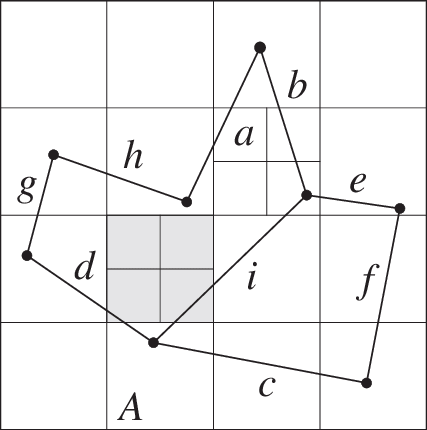
\includegraphics[width=0.3\textwidth]{imatges/pm_quadtree.png}\par\vspace{1cm}
	\caption{PM Quadtree}
	\label{fig:pm_quadtree}
\end{figure}

Un \textit{PM QuadTree} (\textit{Figura \ref{fig:pm_quadtree}}) és una estructura de dades molt utilitzada en informàtica gràfica i es basa en una descomposició jeràrquica dels objectes de l’espai que descriuen. Es crea a partir d’una caixa englobant de forma quadrada que conté tots els polígons (coordenades) que s’estan descrivint. Aquest espai que hi ha, es divideix en quatre quadrats iguals (quadrants) generant així quatre fills que, juntament amb el pare, formen un arbre 4‐àri. Tot seguit es reparteixen tots els polígons en el fill corresponent depenent de la seva posició. Aquest procés es va repetint fins que cada node concret conté tan sols un polígon.

L’ordre que s’estableix per a assignar quin número té cada fill és segons l’ordre de \textit{Morton} (veure \textit{Figura \ref{fig:quadtree_ordre_de_morton}}), que dóna prioritat al fill superior‐esquerre.

\begin{figure}[H]
	\centering
	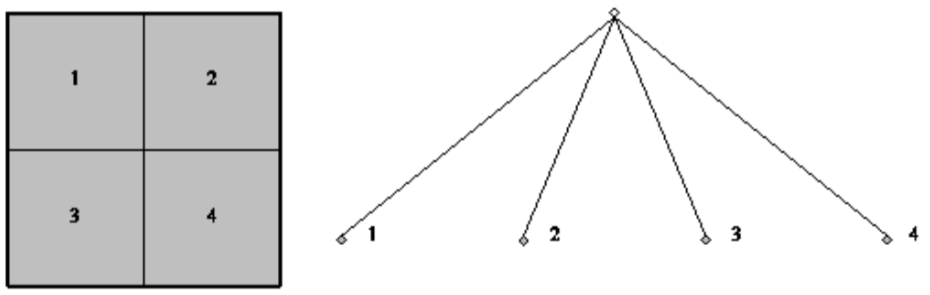
\includegraphics[width=0.7\textwidth]{imatges/quadtree_ordre_de_morton.png}\par\vspace{1cm}
	\caption{QuadTree: Ordre de Morton}
	\label{fig:quadtree_ordre_de_morton}
\end{figure}

A la \textit{Figura \ref{fig:exemple_pm_quadtree}} es pot veure un exemple molt senzill d’un QuadTree amb 5 poligons juntament amb el seu arbre generat.

\begin{figure}[H]
	\centering
	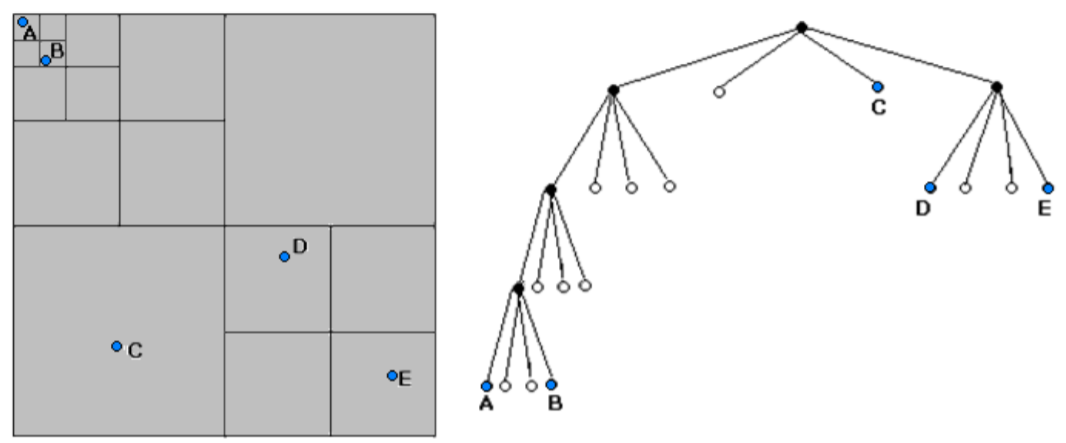
\includegraphics[width=0.8\textwidth]{imatges/exemple_pm_quadtree.png}
	\caption{Exemple PM QuadTree}
	\label{fig:exemple_pm_quadtree}
\end{figure}

%EXPLICACIÓ DE L'ALGORTME PM QUADTREE (MERIEM)

%Un exemple de l'aplicació d'aquesta estructura es pot veure en la següent \textit{Figura \ref{fig:poligon_pm_quadtree}}:

%\begin{figure}[H]
	%\centering
	%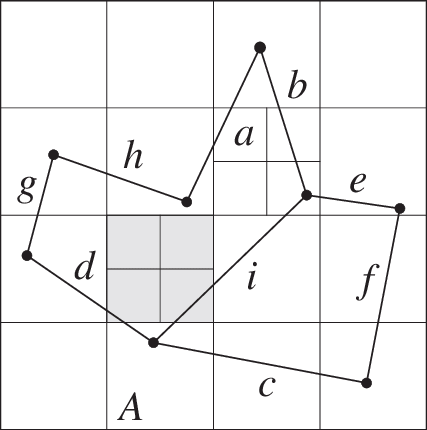
\includegraphics[width=0.5\textwidth]{imatges/pm_quadtree_exemple.png}\par\vspace{1cm}
	%\caption{Poligon emmagatzemat en un PM Quadtree}
	%\label{fig:poligon_pm_quadtree}
%\end{figure}

%FALTA EXPLICACIÓ DE L'EXEMPLE AMB L'ALGORISME (MERIEM)

Un cop es té creada l'estructura, s'avaluarà cada un dels punts per veure en quina regió està. Si aquesta regió conté part d'un obstacle s'haurà de comprovar si el punt està o no dins d'aquest. Si el punt no es troba dins d'un obstacle, es considerarà una dada vàlida i es posicionarà a sobre d'una grid, de manera que, a la grid tindrem posicionades totes les dades vàlides. Podem veure a la següent \textit{Figura \ref{fig:grid_amb_punts}} un exemple de com seria la grid.

\begin{figure}[H]
	\centering
	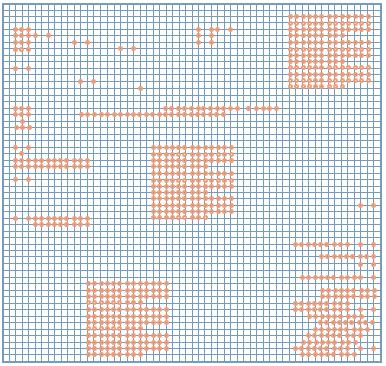
\includegraphics[width=0.45\textwidth]{imatges/grid_amb_punts.png}
	\caption{Grid amb Punts}
	\label{fig:grid_amb_punts}
\end{figure}

\subsection{Assignar un pes a cada atracció}
El pes d'una atracció es definirà a partir de la quantitat de gent que ha pujat a aquesta. Per cada pivot, s'assigna un pes $p_{i}$ tal que:
 
$$p_{i} = \frac{q_{i}}{t}$$

on:
\begin{itemize}
	\item $q_{i}$ és la quantitat de gent que ha pujat a l'atracció $i$.
	\item $t$ és el total de gent.
\end{itemize}

En la següent \textit{Figura \ref{fig:mapa_areas_totals}} es pot veure el mapa amb els pesos totals per a cada una de les atraccions.

\begin{figure}[H]
	\centering
	\includegraphics[width=0.8\textwidth]{imatges/pesos_totals.png}\par\vspace{1cm}
	\caption{Pesos de cada atracció}
	\label{fig:mapa_areas_totals}
\end{figure}

En la següent \textit{Figura \ref{fig:mapa_areas}} es pot veure el mapa amb la proporció de pesos per a cada una de les atraccions.

\begin{figure}[H]
	\centering
	\includegraphics[width=0.8\textwidth]{imatges/pesos.png}\par\vspace{1cm}
	\caption{Proporció de pesos de cada atracció}
	\label{fig:mapa_areas}
\end{figure}

\subsection{Dividir el mapa en àrees \label{arees}}
A partir del pes de cada atracció (ubicat en l'entrada d'aquesta), es poden seguir diferents estratègies per calcular la regió d'influència per cada una de les atraccions a partir del nombre de persones que hi ha al voltant.

\subsubsection{Estratègies}
Algunes d'aquestes estratègies són:
\begin{itemize}
	\item Utilitzar un diagrama de \textit{Voronoi} per definir la regió d'interès de cada atracció (cada persona dins d'aquesta àrea computa 1).
	\item Utilitzar l'estratègia del punt anterior, i per cada atracció, per cada una de les àrees no definides pel pivot, computar les persones que hi ha com $\frac{1}{1+d}$ on $d$ correspon a la distància en metres des de la persona a l'entrada de l'atracció.
	\item Utilitzar l'estratègia del punt anterior, però aquesta vegada comptant la distància ($d$) des de la persona al segment que defineix l'àrea regida pel pivot.
	\item Utilitzar diagrames de \textit{Voronoi} de nivell amb capa ($k$ on $2 \le k \le n$ i $n$ és el nombre d'atraccions), el diagrama de primer nivell defineix la regió de màxim interés de l'atracció (computant 1 per cada persona) i les capes $k-1$ \textbf{capes superposades}, determinen zones d'interès però no tan importants (computen $\frac{1}{k}$ per cada persona).
\end{itemize}

Segons l'estratègia que es volgués seguir, s'obtindria una distribució en àrees o un altre. En aquest cas, s'ha optat per utilitzar l'última proposta amb una $k = 2$, ja que es creu que és una bona aproximació pel problema que es vol resoldre. 

Un cop entès que és un diagrama de \textit{Voronoi} sobre el pla (veure Annex \ref{ann:dvoronoi}), podem aplicar els mateixos conceptes sobre aquest projecte. 

A partir de la funció distància de cada punt es pot obtenir diferents diagrames de \textit{Voronoi}: el més proper i el segon més proper. 

Per trobar els diferents diagrames de \textit{Voronoi}, cal definir de quina manera es calcularan les distàncies entre dos punts. Per calcular la distància entre un punt i un pivot s'utilitzarà l'\textbf{alogirtme A*} (veure Annex \ref{ann:a_star}) per cada punt de la grid, de manera que el primer pivot trobat es considera el punt generador més proper i el segon trobat, es considera el segon punt generador més proper.

Des de cada punt situat a la grid es buscarà el primer i segon pivot més proper tenint en compte que a la grid hi han camins habilitats i no habilitats (els camins no habilitats corresponen als camins on es troba un obstacle). Per això, abans d'aplicar A*, aplicarem l'\textbf{algoritme Dijkstra} sobre la grid començant des d'un pivot per eliminar tots els camins que no estan habilitats, és a dir, que hi hagin obstacles.

\subsubsection{Diagrama de \textit{Voronoi} de primer nivell} 

En la següent \textit{Figura \ref{fig:diagrama_voronoi_ordre_1}} es pot veure una possible representació del diagrama de \textit{Voronoi} d'ordre 1 per l'escenari plantejat.

\begin{figure}[H]
	\centering
	\includegraphics[width=0.75\textwidth]{imatges/diagrama_voronoi_ordre_1.png}
	\caption{Diagrama de \textit{Voronoi} d'ordre 1}
	\label{fig:diagrama_voronoi_ordre_1}
\end{figure}

\subsubsection{Capa de \textit{Voronoi} de primer nivell capa 2}
Per afinar més els càlculs, es vol calcular la capa 2 del diagrama de \textit{Voronoi} de primer nivell, i a partir d'aquesta obtenir una aproximació de la influència de les persones que estan pròximes a les àrees definides en el primer nivell.

Per obtenir la capa 2, cal realitzar l'algoritme del \textbf{diagrama de \textit{Voronoi} de primer nivell capa 2} utilitzant, com a pivot del diagrama de \textit{Voronoi}, el segon pivot més proper.

%En la següent figura (\ref{fig:diagrama_voronoi_ordre_2}) es pot veure el diagrama de \textit{Voronoi} de primer nivell capa 2, el qual superposant-lo amb el diagrama de \textit{Voronoi} de primer nivell, s'obtindria la capa de superposició que es vol.

%Superposant el diagrama de \textit{Voronoi} de segon nivell amb el diagrama de \textit{Voronoi} de primer nivell, s'obtindria la capa de superposició que es vol.

%\textbf{Falta posar els poligons que regeixen les zones prohibides, rius, llacs, les propies atraccions...}

%\begin{figure}[H]
	%\centering
	%\includegraphics[width=1\textwidth]{imatges/diagrama_voronoi_ordre_2.png}\par\vspace{1cm}
	%\caption{Diagrama de \textit{Voronoi} d'ordre 2}.
	%\label{fig:diagrama_voronoi_ordre_2}
%\end{figure}

\subsection{Definir les zones candidates}
Un cop es disposa de la regió d'influència de cada atracció (veure Secció \ref{arees}). Es vol fer el posicionament dels restaurants, però abans, cal que la direcció del parc proporcioni un mapa tot indicant quines són les possibles ubicacions per aquests restaurants. En la següent \textit{Figura \ref{fig:zones_candidates}} es mostra un possible mapa.

\begin{figure}[H]
	\centering
	\includegraphics[width=0.8\textwidth]{imatges/possibles_ubicacions.png}
	\caption{Mapa amb les possibles ubicacions}
	\label{fig:zones_candidates}
\end{figure}

\subsection{Ubicar els restaurants}
En aquest punt, la direcció ha de proporcionar una llista amb els restaurants que es volen ubicar amb un valor associat, aquest valor ha de reflectir quant car és cada restaurant.

Una vegada es tenen els restaurants a ubicar i les zones candidates, cal calcular el benefici de cada configuració a partir del benefici de cada restaurant i la influència que rep d'acord a les atraccions que té al voltant.  

Per calcular el benefici de cada candidat:
\begin{itemize}
	\item Es defineix l'àrea circular (de radi predefinit) que cobreix un restaurant
	\item Es calcula l'àrea ponderada del pes dels pivots dels diagrames de \textit{Voronoi} superposats de capa 1 i capa 2
\end{itemize}

A continuació es podrà veure un exemple de com seria aquest càlcul. Se suposa que hi ha un restaurant situat en el diagrama de \textit{Voronoi} resultat de superposar les capes 1 i 2 com es veu a la \textit{Figura \ref{fig:benefici_restaurant}}

\begin{figure}[H]
	\centering
	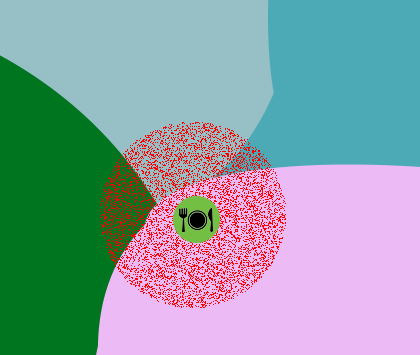
\includegraphics[width=0.5\textwidth]{imatges/benefici_restaurant.png}
	\caption{Restaurant en el diagrama de \textit{Voronoi} superposat de la capa 1 i 2}
	\label{fig:benefici_restaurant}
\end{figure}

$$B_{x} = (A_{1} \cdot P{1} + A_{2} \cdot P_{2} + A_{3} \cdot P_{3} + A_{4} \cdot P_{4}) \cdot C_{i}$$

on:

\begin{itemize}
	\item $B_{x}$: El benefici del restaurant $x$.
	\item $A_{1}$: Àrea de color verd que cobreix el restaurant.
	\item $P_{1}$: Pes de l'àrea de color verd.
	\item $A_{2}$: Àrea de color blau cel que cobreix el restaurant.
	\item $P_{2}$: Pes de l'àrea de color blau cel.
	\item $A_{3}$: Àrea de color blau marí que cobreix el restaurant.
	\item $P_{3}$: Pes de l'àrea de color blau marí.
	\item $A_{4}$: Àrea de color rosa que cobreix el restaurant.
	\item $P_{4}$: Pes de l'àrea de color rosa.
	\item $B_{i}$: Quan car és el restaurant $i$.
\end{itemize}

Una vegada generada totes les combinacions, s'elegirà la que maximitzi el benefici global del parc. En la següent \textit{Figura \ref{fig:mapa_restaurants}} es mostra un exemple d'una possible solució final.

\begin{figure}[H]
	\centering
	\includegraphics[width=1\textwidth]{imatges/solucio.png}
	\caption{Mapa d'atraccions amb les ubicacions dels restaurants}
	\label{fig:mapa_restaurants}
\end{figure}

\clearpage
\section{Pre-processament de dades\label{pd}}
Pel caràcter del problema i per evitar errors, es realitzarà un preprocessament amb els punts recollits, de tal manera que, només es consideraran aquells punts:
\begin{itemize}
	\item S’han recollit dins d’un conjunt de franges horàries que es consideren d'interès pels visitants alhora de buscar un restaurant per menjar. 
	Així doncs, el llistat de franges horàries a considerar és:
	\begin{itemize}
		\item Esmorzar: 9h-10h
		\item Dinar: 12h-14h
		\item Berenar: 17h-18h
		\item Sopar: 20h-22h
	\end{itemize}

	\item No s’hagin recollit a les zones on es troben obstacles. 
	Considerem obstacles a les atraccions, boscos, llacs, etc.
\end{itemize}

Per realitzar-ho, seguirem els següents passos:
\begin{itemize}
	\item Convertir els punts que delimiten el mapa.
	\item Convertir els punts dels pivots i comprovar que estiguin dintre del mapa.
	\item Convertir els punts i les arestes de les zones prohibides.
	\item Convertir els punts de les persones.
	\begin{itemize}
		\item Filtrar els punts per la frange horària. Només es quedaran els punts de les hores que ens interessen.
		\item Convertir els punts filtrats.
	\end{itemize}
\end{itemize}

\textbf{Nota:} Quan es parla de convertir els punts, es fa referència a aplicar l'algorisme de conversió de latitud,longitud a X,Y (veure annex \ref{ann:lat_lon}) per tal de transformar un punt referenciat per (latitud, longitud) en un punt (X, Y).

\clearpage
\section{Treball futur}

\subsection{El càlcul de distàncies}
Es podria mirar de realitzar el càlcul de distàncies amb la programació en paral·lel. El càlcul de distàncies consisteix en realitzar un Dijkstra per eliminar els obstacles i un A* per fel el càlcul de les distàncies entre un punt i un pivot. Tan en el Dijkstra com A*, com que el càlcul de les distàncies entre un punt i un pivot es poden fer independentment, la programació en paral·lel resulta eficaç per millorar l'eficiència del càlcul.

\subsection{El càlcul dels diagrames de Voronoi}
La construcció dels diagrames de Voronoi es comú fer-ho amb la estructura de la triangulació Delaunay. La triangulació Delaunay es pot realitzar amb algoritmes en paral·lel, per tant, es podria realitzar la construcció dels dos diagrames de Voronoi mitjançant la programació en paral·lel.

\subsection{El càlcul de la importància d'una regió}
Pel càlcul de la importància d'una regió es podria tenir en consideració diferents criteris, com per exemple, l'edat dels usuaris, si van en grup, el tipus d'atracció on pugen. Es podria aplicar tècniques per aprofitar l'informació rebuda amb les \textit{Magic Bands}.

\clearpage
\section{Conclusions}

L'objectiu principal d'aquest projecte és \textbf{fer la distribució dels restaurants amb l'objectiu de ubicar aquells que són més cars en les zones més freqüentades}, per això, es parteix de la informació d'un parc d'atracció similar en el qual s'han recollit les dades dels visitants del parc a través de les \textit{Magic Bands}. L'objectiu d'aquest projecte ha estat complert satisfactòriament. 

Aquest objectiu, com s’ha pogut comprovar, ha estat complert de forma satisfactòria. Tot el conjunt de requeriments definits des d’un principi han estat assolits al final.

Amb el desenvolupament d’aquest treball hem pogut veure la complexitat dels problemes de dades espaials. El que en principi semblen problemes simples tenen solucions bastant complicades de trobar.

Finalment creiem que la solució donada compleix els requeriments inicials i dona resposta al problema plantejat, però ens hagués agradat aprofundir una mica més tècnicament en l’algoritme.

\clearpage
\begin{thebibliography}{9}
\bibitem{cert1} \textsc{Gizmodo.com.}, \textit{How I Let Disney Track My Every Move}, 2017. 
\\\textcolor{blue}{\url{https://gizmodo.com/how-i-let-disney-track-my-every-move-1792875386}}	
\bibitem{cert2} \textsc{Okabe, A.}; \textsc{Boots, B.}; \textsc{Sugihara, K.}, \textit{Spatial tessellations. Concepts and Aplicattións of \textit{Voronoi} Diagrams 2ºe.d}. 
\\\textcolor{blue}{\url{http://www.gbv.de/dms/ilmenau/toc/119618044.PDF}}
\bibitem{cert3} \textsc{Abellanas, B.}; \textsc{Abellanas, M.}; \textsc{Vilas, C.}, \textit{Modelización de bosques mediante diagramas de \textit{Voronoi}}, 2018. 
\\\textcolor{blue}{\url{https://www.infor.uva.es/egc07/articulos/28.pdf}}
\bibitem{cert4} \textsc{Moya Carrasco, Á.}, \textit{Generación de trayectorias en tiempo real a partir de diagramas de \textit{Voronoi}}, 2016. \\\textcolor{blue}{\url{https://idus.us.es/xmlui/bitstream/handle/11441/44404/TFG_Angel_Moya_Carrasco.pdf?sequence=1&isAllowed=y}}
\bibitem{cert5} \textsc{Trinchet Almaguer, D}; \textsc{Pérez Rosés, H.}, \textit{Algoritmo para solucionar el problema inverso generalizado de \textit{Voronoi}}, 2007. 
\\\textcolor{blue}{\url{http://www.redalyc.org/pdf/3783/378343634005.pdf}}
\bibitem{cert6} \textsc{García, O.}, \textit{The state-space approach in growth modelling}, 1994. 
\\\textcolor{blue}{\url{https://www.researchgate.net/publication/237870252_The_state-space_approach_in_growth_modelling}}
\bibitem{cert7} \textsc{ABC.}, \textit{El diagrama de \textit{Voronoi}, la forma matemática de dividir el mundo}, 2017. 
\\\textcolor{blue}{\url{https://www.abc.es/ciencia/abci-diagrama-voronoi-forma-matematica-dividir-mundo}}
\\\textcolor{blue}{\url{-201704241101_noticia.html}}
\end{thebibliography}

\clearpage
\appendix
\section{Diagrames de Voronoi \label{ann:dvoronoi}}
Quan es parla dels diagrames de \textit{Voronoi} es fa referència a una estructura geomètrica que representa informació de proximitat sobre un conjunt de punts. Els diagrames de \textit{Voronoi} són una de les estructures fonamentals dins de la Geometria Computacional, d’alguna manera emmagatzemen tota la informació referent a la proximitat entre punts.

Però què és un diagrama de \textit{Voronoi}? Per tal d’entendre millor el concepte introduirem els diagrames de \textit{Voronoi} sobre el pla.

En la següent \textit{Figura \ref{fig:regio_voronoi}} podem veure que el punt $x$ està dins de la regió de punts més propers a $p$. Aquesta regió és la regió de \textit{Voronoi} del punt $p$, i $p$ és el punt generador de la regió.

\begin{figure}[H]
	\centering
	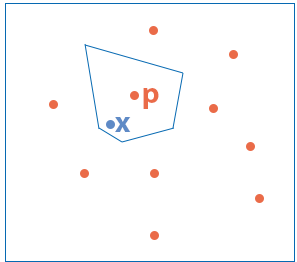
\includegraphics[width=0.28\textwidth]{imatges/regio_voronoi.png}
	\caption{Regió \textit{Voronoi}}
	\label{fig:regio_voronoi}
\end{figure}

La unió de totes les regions de \textit{Voronoi} formen el diagrama de \textit{Voronoi}, tal i com es pot veure a la \textit{Figura \ref{fig:diagrama_voronoi}}

\begin{figure}[H]
	\centering
	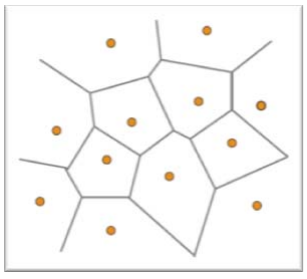
\includegraphics[width=0.28\textwidth]{imatges/diagrama_voronoi.png}
	\caption{Diagrama de \textit{Voronoi}}
	\label{fig:diagrama_voronoi}
\end{figure}

\clearpage
\section{Algoritme A*\label{ann:a_star}}
La primera operació a realitzar, és dividir l'espai en caselles. En el nostre cas les caselles són quadrades, però realment es pot adaptar l'algoritme de dividir l'espai de la forma que es desitgi (triangles, hexàgons, etc.). A partir d'ara cada casella serà una cel·la espacial (es crearà una estructura de dades que la representi) relacionada amb els seus adjacents i amb el seu "pare"; el pare serà la cel·la per la qual hem arribat a tenir en compte l'actual com a possible candidata a formar part del camí final.

Aspectes a tenir en consideració:

\begin{enumerate}
	\item Tenir dues llistes de cel·les: una \textbf{oberta} i una \textbf{tancada}. A la llista \textbf{oberta} anirem introduint cel·les que hem d'avaluar, per veure si són bones candidates a formar part del camí final. A la llista \textbf{tancada} introduirem les cel·les ja avaluades.

	\item L'\textbf{avaluació de les cel·les} es fa en base a dos factors: la longitud del camí més curt per arribar des del punt d'origen a la cel·la actual, i l'estimació del camí més curt que podria quedar per arribar a la destinació. L'estimació pel destí es fa usant una funció \textbf{heurística}, en concret se sol usar la \textbf{Distància Manhattan}, que essencialment consisteix a explorar totes les cel·les que separen el destí vertical i horitzontalment, sense moviments diagonals; com si estiguéssim recorrent \say{pomes} en una gran ciutat i no poguéssim travessar-les, només vorejar-les (d'aquí ve el nom).
\end{enumerate}

L'algoritme té diferents passos:

\begin{enumerate}
	\item Afegim la cel origen a la llista oberta.
	\item Agafem el primer element de la llista oberta i el traiem i l'inserim en la llista tancada.
	\item Agafem les cel·les adjacents a la cel·la extreta.
	\item Per a cada cel·la adjacent:
	\begin{itemize}
		\item Si la cel·la és el destí, hem acabat. Recorrem inversament la cadena de pares fins a arribar a l'origen per obtenir el camí.
		\item Si la cel·la representa un mur o terreny infranquejable; la ignorem.
		\item Si la cel·la ja és a la llista tancada, la ignorem.
		\item Si la cel·la ja és a la llista oberta, comprovem si la seva nova G (ho veurem més endavant) és millor que l'actual, i en aquest cas recalculem factors (ho veurem més endavant) i posem com a pare de la cel·la, la cel·la extreta. En cas que no sigui millor, la ignorem.
		\item Per a la resta de cel·les adjacents, els establim com a pare la cel·la extreta i recalculem factors. Després les afegim a la llista oberta.
	\end{itemize}
	\item Ordenem la llista oberta. La llista oberta és una llista ordenada de forma ascendent en funció del factor F de les cel·les.
	\item Tornar al pas 1.
\end{enumerate}

Factors a tenir en consideració:

Cada cel·la té 3 factors. G, H i F.

\begin{itemize}
	\item \textbf{G:} És el cost d'anar des de la cel·la origen fins a l'actual. Cada vegada que ens moguem un pas en horitzontal o vertical, afegirem 10 punts de cost. Cada vegada que ens moguem en diagonal, afegirem 14. Per què 14? Perquè encara que geomètricament la proporció exacta hauria de ser 14,14213 ($\sqrt{10 * 10 + 10 * 10}$), 14 és una bona aproximació sencera que ens farà guanyar velocitat en evitar l'ús de coma flotant.

	\item \textbf{H:} És la distància mínima i optimista, sense usar diagonals, que resta fins a la destinació. L'heurística basada en Distància Manhattan de la qual hem parlat abans.

	\item \textbf{F:} És la suma de \textbf{G} i \textbf{H}.
\end{itemize}

\clearpage
\section{Algorisme latitud longitud \label{ann:lat_lon}}

%public class MapService {
    // CHANGE THIS: the output path of the image to be created
    private static final String IMAGE_FILE_PATH = "/some/user/path/map.png";

    // CHANGE THIS: image width in pixel
    private static final int IMAGE_WIDTH_IN_PX = 300;

    // CHANGE THIS: image height in pixel
    private static final int IMAGE_HEIGHT_IN_PX = 500;

    // CHANGE THIS: minimum padding in pixel
    private static final int MINIMUM_IMAGE_PADDING_IN_PX = 50;

    // formula for quarter PI
    private final static double QUARTERPI = Math.PI / 4.0;

    // some service that provides the county boundaries data in longitude and latitude
    private CountyService countyService;

    public void run() throws Exception {
        // configuring the buffered image and graphics to draw the map
        BufferedImage bufferedImage = new BufferedImage(IMAGE_WIDTH_IN_PX,
                                                        IMAGE_HEIGHT_IN_PX,
                                                        BufferedImage.TYPE_INT_RGB);

        Graphics2D g = bufferedImage.createGraphics();
        Map<RenderingHints.Key, Object> map = new HashMap<RenderingHints.Key, Object>();
        map.put(RenderingHints.KEY_INTERPOLATION, RenderingHints.VALUE_INTERPOLATION_BICUBIC);
        map.put(RenderingHints.KEY_RENDERING, RenderingHints.VALUE_RENDER_QUALITY);
        map.put(RenderingHints.KEY_ANTIALIASING, RenderingHints.VALUE_ANTIALIAS_ON);
        RenderingHints renderHints = new RenderingHints(map);
        g.setRenderingHints(renderHints);

        // min and max coordinates, used in the computation below
        Point2D.Double minXY = new Point2D.Double(-1, -1);
        Point2D.Double maxXY = new Point2D.Double(-1, -1);

        // a list of counties where each county contains a list of coordinates that form the county boundary
        Collection<Collection<Point2D.Double>> countyBoundaries = new ArrayList<Collection<Point2D.Double>>();

        // for every county, convert the longitude/latitude to X/Y using Mercator projection formula
        for (County county : countyService.getAllCounties()) {
            Collection<Point2D.Double> lonLat = new ArrayList<Point2D.Double>();

            for (CountyBoundary countyBoundary : county.getCountyBoundaries()) {
                // convert to radian
                double longitude = countyBoundary.getLongitude() * Math.PI / 180;
                double latitude = countyBoundary.getLatitude() * Math.PI / 180;

                Point2D.Double xy = new Point2D.Double();
                xy.x = longitude;
                xy.y = Math.log(Math.tan(QUARTERPI + 0.5 * latitude));

                // The reason we need to determine the min X and Y values is because in order to draw the map,
                // we need to offset the position so that there will be no negative X and Y values
                minXY.x = (minXY.x == -1) ? xy.x : Math.min(minXY.x, xy.x);
                minXY.y = (minXY.y == -1) ? xy.y : Math.min(minXY.y, xy.y);

                lonLat.add(xy);
            }

            countyBoundaries.add(lonLat);
        }

        // readjust coordinate to ensure there are no negative values
        for (Collection<Point2D.Double> points : countyBoundaries) {
            for (Point2D.Double point : points) {
                point.x = point.x - minXY.x;
                point.y = point.y - minXY.y;

                // now, we need to keep track the max X and Y values
                maxXY.x = (maxXY.x == -1) ? point.x : Math.max(maxXY.x, point.x);
                maxXY.y = (maxXY.y == -1) ? point.y : Math.max(maxXY.y, point.y);
            }
        }

        int paddingBothSides = MINIMUM_IMAGE_PADDING_IN_PX * 2;

        // the actual drawing space for the map on the image
        int mapWidth = IMAGE_WIDTH_IN_PX - paddingBothSides;
        int mapHeight = IMAGE_HEIGHT_IN_PX - paddingBothSides;

        // determine the width and height ratio because we need to magnify the map to fit into the given image dimension
        double mapWidthRatio = mapWidth / maxXY.x;
        double mapHeightRatio = mapHeight / maxXY.y;

        // using different ratios for width and height will cause the map to be stretched. So, we have to determine
        // the global ratio that will perfectly fit into the given image dimension
        double globalRatio = Math.min(mapWidthRatio, mapHeightRatio);

        // now we need to readjust the padding to ensure the map is always drawn on the center of the given image dimension
        double heightPadding = (IMAGE_HEIGHT_IN_PX - (globalRatio * maxXY.y)) / 2;
        double widthPadding = (IMAGE_WIDTH_IN_PX - (globalRatio * maxXY.x)) / 2;

        // for each country, draw the boundary using polygon
        for (Collection<Point2D.Double> points : countyBoundaries) {
            Polygon polygon = new Polygon();

            for (Point2D.Double point : points) {
                int adjustedX = (int) (widthPadding + (point.getX() * globalRatio));

                // need to invert the Y since 0,0 starts at top left
                int adjustedY = (int) (IMAGE_HEIGHT_IN_PX - heightPadding - (point.getY() * globalRatio));

                polygon.addPoint(adjustedX, adjustedY);
            }

            g.drawPolygon(polygon);
        }

        // create the image file
        ImageIO.write(bufferedImage, "PNG", new File(IMAGE_FILE_PATH));
    }
}

\lstinputlisting[language=java]{codi/convert_lat_long_x_y.txt}
\end{document}


